\documentclass[.../Dokumentation.tex]{subfiles}
\begin{document}
\subsection{Darstellung}\label{sec-ita2-visualization}
Die im Zuge der vorangegangenen Iteration erdachte Umsetzung einer abstrakteren 
Darstellungsweise wurde in diesem Arbeitsschritt vorangetrieben.\\
Anhand eines ersten Papierprototypen, zu sehen in Abbildung 
\ref{fig-tree-paper}, wurde begonnen, das bereits bei der Herstellung der 
Fahrzeugprototypen gewonnene Wissen auf die Schaffung eines druckfähigen 
Baummodels anzuwenden.
\begin{figure}[H]
\begin{center}
    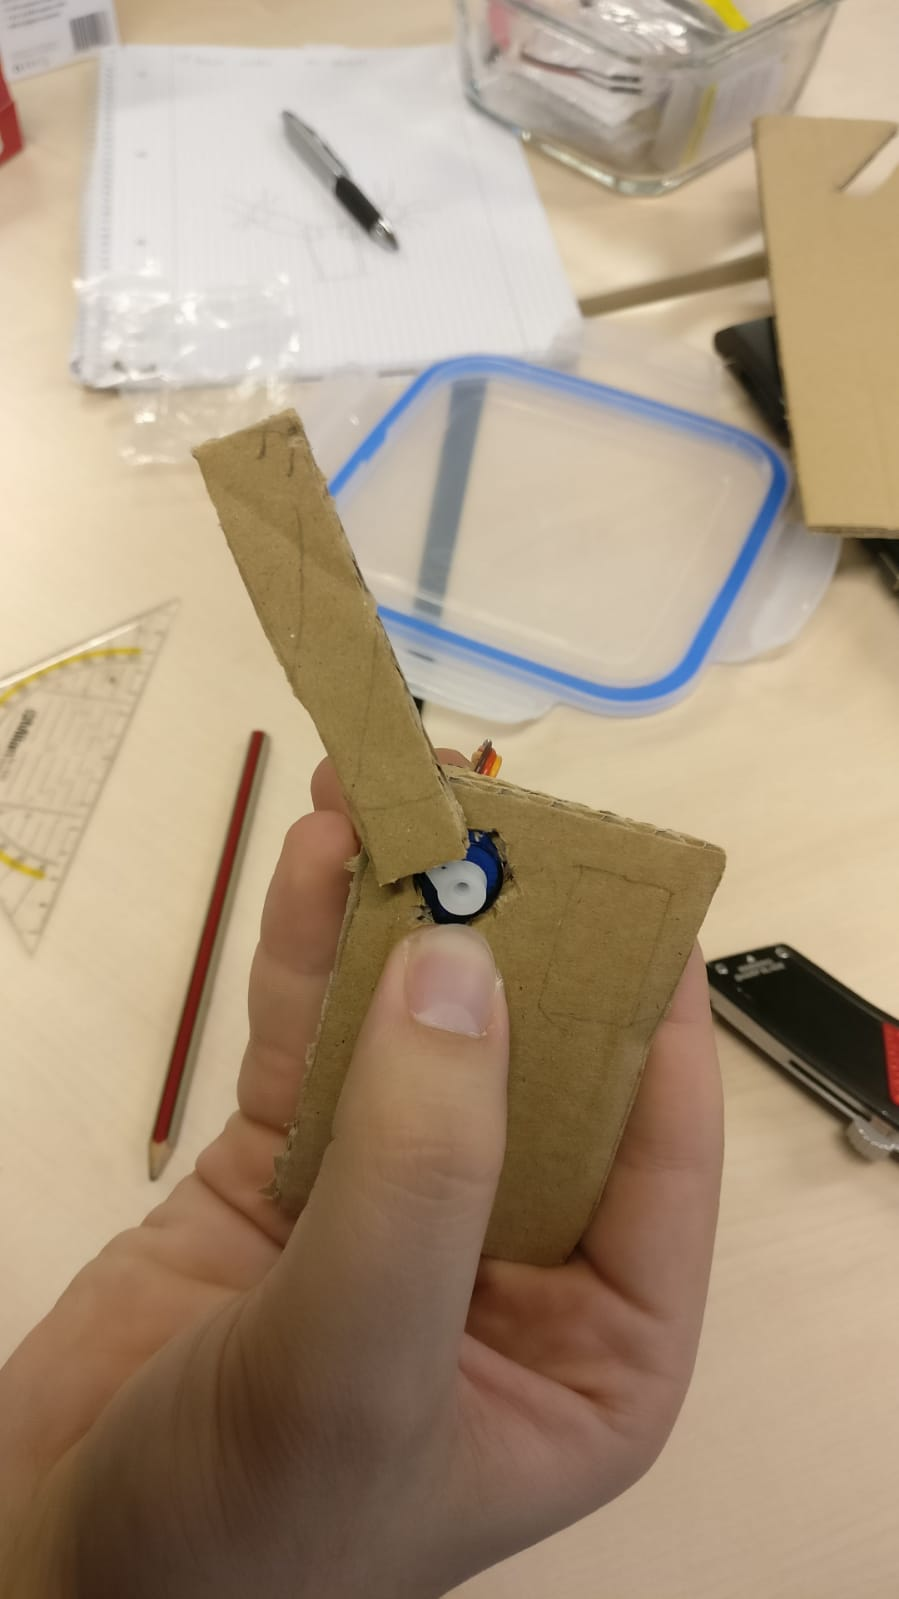
\includegraphics[
        width=0.5\linewidth,
    ]{imgs/tree_paper.jpg}
    \caption{Papierprototyp des Baums}
    \label{fig-tree-paper}
\end{center}
\end{figure}
\noindent
Mit den Maßen der Servomotoren als Referenz wurde mit den Modellierungsarbeiten 
begonnen. Ebendiese Maße bedingten jedoch verhältnismäßig dicke Äste in der 
geplanten Umsetzung des Baums. 
Die daraus resultierenden Dimensionen, insbesondere in die Tiefe, zeigt 
Abbildung \ref{fig-tree-side}.
\begin{figure}[H]
\begin{center}
    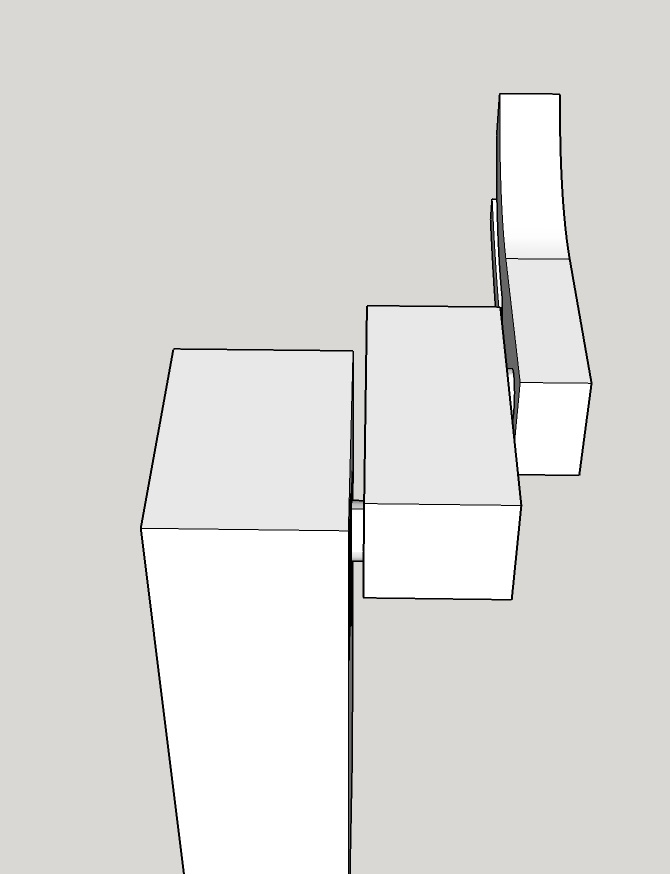
\includegraphics[
        width=0.5\linewidth,
    ]{imgs/tree_side.jpg}
    \caption{Dimensionen des Baummodels}
    \label{fig-tree-side}
\end{center}
\end{figure}
\end{document}